\documentclass{article}
\usepackage[utf8]{inputenc}
\usepackage[english]{babel}
\usepackage{amsmath}% http://ctan.org/pkg/amsmath
\usepackage{listings}
\usepackage{graphicx}
\usepackage{comment}
\usepackage{float}
\usepackage{biblatex}
\usepackage{lscape}
\usepackage{csquotes}
\usepackage{multirow}
\addbibresource{bibliography.bib}
\usepackage[a4paper,pdftex,bottom=20mm, width=160mm]{geometry} % A4paper margins
\setlength{\parindent}{0pt} % Tar bort indenteringen på paragrafer 
\setlength{\parskip}{1em}


\title{
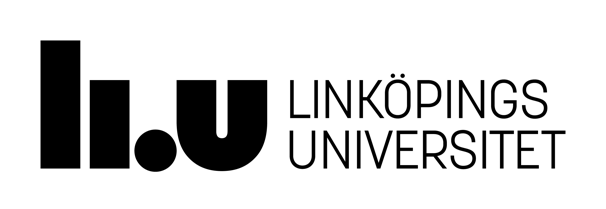
\includegraphics[scale=1.5]{liu_logga.png} \\
\vspace{2.0cm} \textbf{Customer Requirements Specification} \\
 \endgraf\rule{\textwidth}{.4pt}
  \large \textbf{TDDC88 - Project}\\
   }
   
   
\author{William Eriksson, Alina Wåhlberg, Gustav Gaunitz \& Melker Forsberg}
\date{\today}

\begin{document}

\maketitle


\newpage
\tableofcontents
\newpage

% Here you will find information about the file
\section{Introduction}


\subsection{Purpose}



\subsection{Scope}


\subsection{Definitions, acronyms and abbreviation}

\newpage

% Here you'll find information about the project
\section{Overall Description}

\subsection{Product perspective}

\newpage

% Here you'll find information about requirements
\section{Specific requirements}


\newpage
¨% Here you'll find additional relevant info about the project
\section{Supporting information}

\newpage
\printbibliography

\end{document}
